% !TEX root = ../../main.tex


\begin{figure}[!htb]
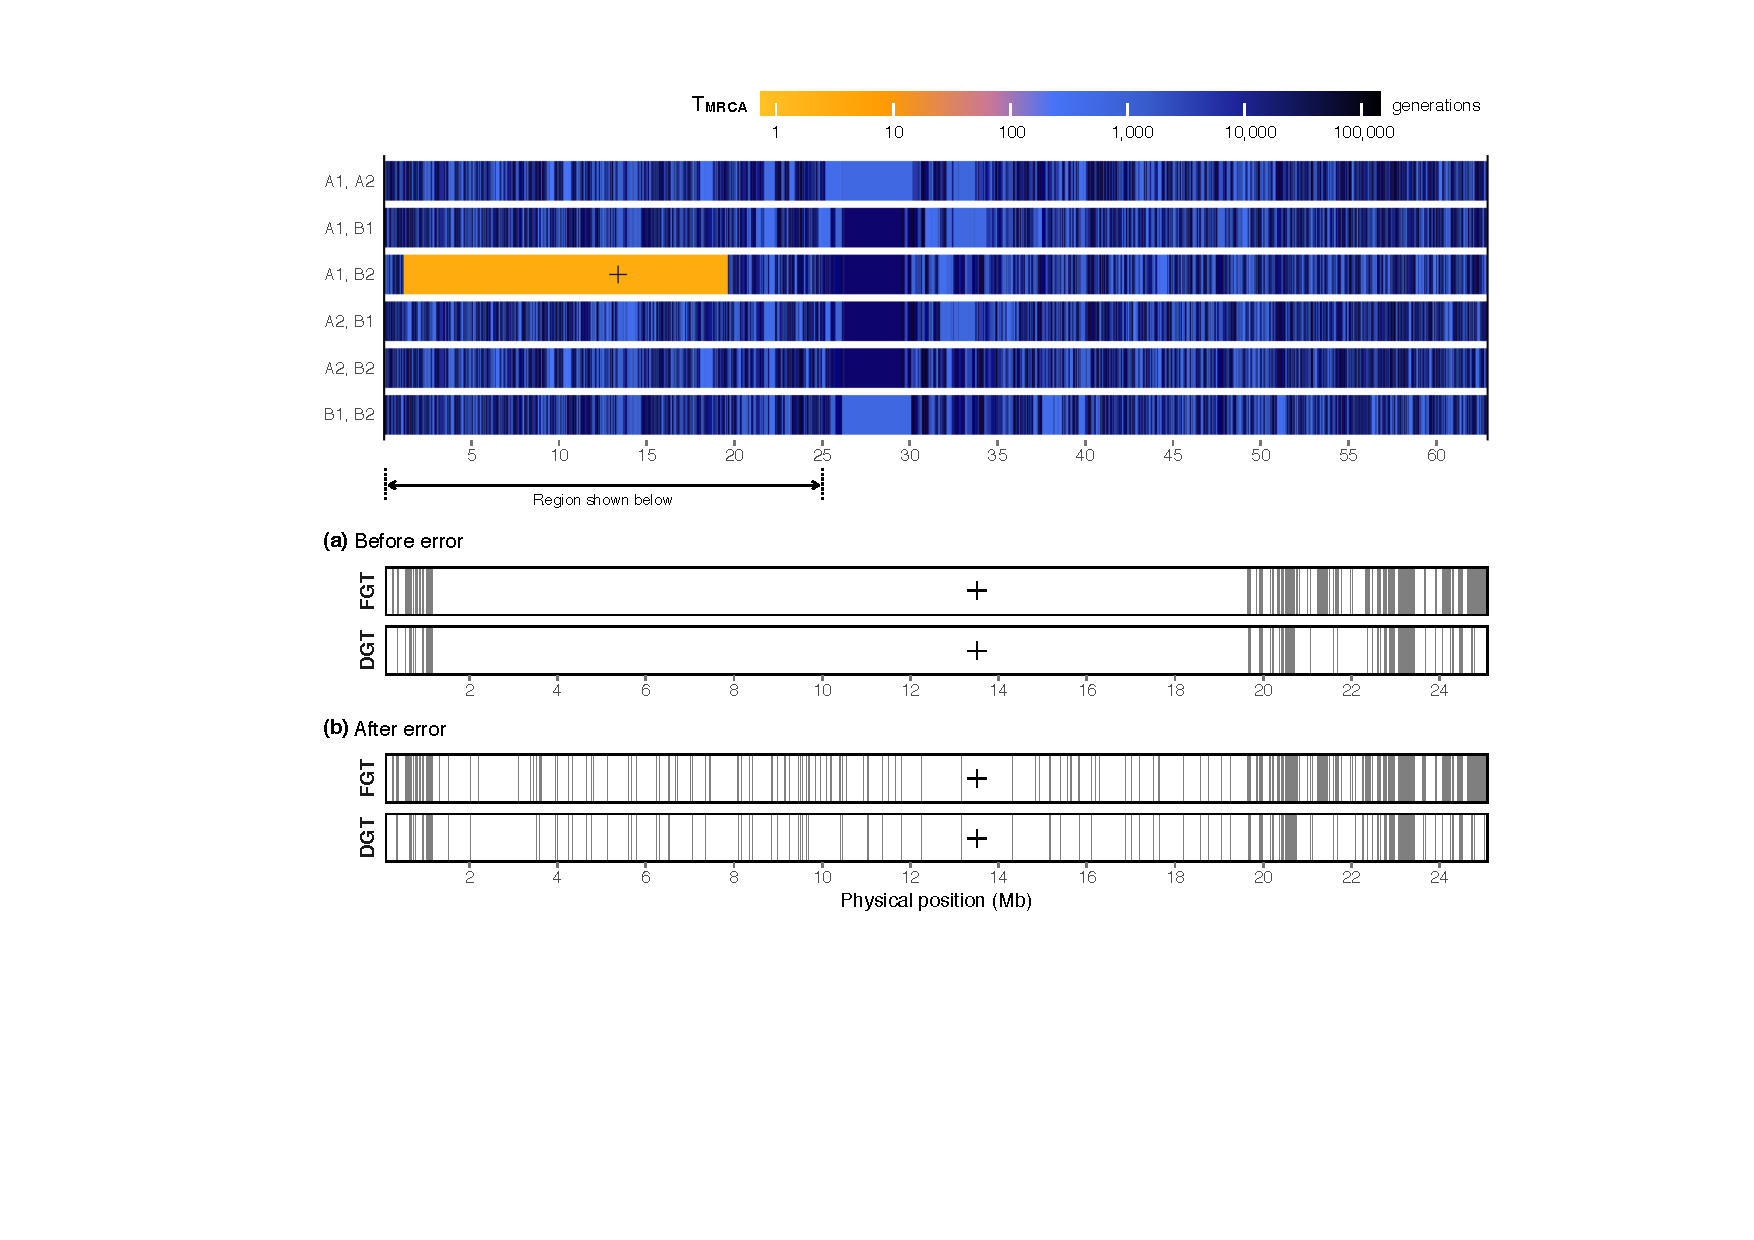
\includegraphics[width=\textwidth]{./img/ch4/full_ibd_error}
\Caption{Example of the effect of genotype error on IBD detection}
{Using simulated data, the underlying IBD structure for all \n{6} possible pairs of the \n{4} chromosomes in \n{2} individuals is shown (\emph{top}); determined from simulation records.
The pair of individuals was randomly selected among those sharing a rare allele which identified recent haplotype sharing by descent.
The figure shows the ``mosaic'' of IBD segments along the sequence of the simulated chromosome; distinguished by the \gls{tmrca}.
The focal shared allele is indicated at the pair of chromosomes sharing that allele (\emph{cross}).
Data were compared before \textbf{(a)} and after \textbf{(b)} the inclusion of empirically determined genotype error.
In each dataset, the \gls{fgt} and \gls{dgt} were used to detect breakpoints to the left and right-hand side of the target position.
The first breakpoints to each side delimit the detected IBD interval; here, all breakpoint following first detection are shown.
Data were simulated using \texttt{msprime} (see \ctref{sec:msprime}).}
{fig:full_ibd_error}
\end{figure}
